\section[Multiplicateurs de Lagrange]{Multiplicateurs de Lagrange}

\begin{frame}{Formulation d'un problème d'optimisation}
	Un problème d'\textbf{optimisation} consiste à chercher la valeur maximale, ou minimale, d'une fonction $f(x)$ ou, alternativement, à chercher la valeur de l'\textbf{argument} $x$ maximisant, ou minimisant, cette même fonction. Supposons que nous cherchions l'argument $x$ d'une fonction $f$ que l'on souhaite maximiser, le problème s'écrit donc: \\
	\begin{equation}
		\begin{cases}
			f: \R^p \to \R \\
			\argmax{x \in \R^p} f(x)
		\end{cases}
		\nonumber
	\end{equation}
\end{frame}

\begin{frame}{Formulation d'un problème d'optimisation sous contraintes}
	Un problème d'optimisation sous contraintes force l'argument $x$ à satisfaire certaines conditions afin d'être une solution \textbf{admissible} au problème. Une telle condition est, par exemple, une \textbf{contrainte d'égalité} comme $g(x) = 0$. Si on ajoute ce type de contrainte à notre problème ci-avant, la formalisation devient:
	\begin{equation}
		\begin{cases}
			f: \R^p \to \R \\
			g: \R^p \to \R \\
			\argmax{x \in \R^p} f(x) \quad \text{sous contrainte} \quad g(x) = 0
		\end{cases}
		\nonumber
	\end{equation}
	\pause
	Note: dans les formulations suivantes, la mention \textit{sous contrainte} sera simplement abrégée en \textit{s.c.}
\end{frame}

\begin{frame}{\'Enoncé des Multiplicateurs de Lagrange}
	\begin{block}{Théorème: Multiplicateurs de Lagrange}
		Soit un problème de recherche d'argument $x \in \R^p$ maximisant une fonction $f: \R^p \to \R$ sous contrainte d'égalité $g(x) = 0$ avec $g: \R^p \to \R$:
		\begin{equation}
			\argmax{x}f(x) \quad \text{s.c.} \quad g(x) = 0
			\nonumber
		\end{equation}
		On introduit une fonction appelée \textbf{Lagrangien}, notée $\mathcal{L}: \R^p \times \R \to \R$, et un \textbf{multiplicateur}, noté $\lambda \in \R$ tels que:
		\begin{equation}
			\mathcal{L}(x, \lambda) = f(x) - \lambda g(x)
			\nonumber
		\end{equation}
		Une solution à ce problème d'optimisation sous contrainte $(x^*, \lambda^*)$ est obtenue lorsque les dérivées du Lagrangien s'annulent:
		\begin{equation}
			\begin{cases}
				\nabla_x \mathcal{L}(x^*, \lambda^*) = 0          & \text{condition de stationnarité} \\
				\nabla_{\lambda} \mathcal{L}(x^*, \lambda^*) = 0  & \text{condition d'admissibilité}
				\nonumber
			\end{cases}
		\end{equation}
	\end{block}
\end{frame}

\begin{frame}{Interprétation des Multiplicateurs de Lagrange}
	Dans le théorème précédent:
	\begin{itemize}
		\item $\nabla$ représente l'opérateur \textbf{gradient}:
		\begin{equation}
			\nabla_x = \begin{pmatrix}
				\frac{\partial}{\partial{x_1}} \\
				\frac{\partial}{\partial{x_2}} \\
				\vdots \\
				\frac{\partial}{\partial{x_p}} \\
			\end{pmatrix}; \quad \nabla_{\lambda} = \frac{\partial}{\partial{\lambda}}
			\nonumber
		\end{equation}
		\pause
		\item La première condition de stationnarité garantit que l'on cherche un maximum pour $f$. Elle s'assure également de la colinéarité des gradients $\nabla_x$ de $f(x)$ et de $g(x)$, et donc de la tangence des courbes représentatives des fonctions $f$ et $g$ au point optimal $(x^*, \lambda^*)$.
	\end{itemize}
\end{frame}

\begin{frame}{Interprétation des Multiplicateurs de Lagrange}
	Dans le théorème précédent:
	\begin{itemize}
		\item La seconde condition d'admissibilité garantit que la contrainte $g(x) = 0$ est satisfaite, en effet: $\nabla_{\lambda}\mathcal{L}(x, \lambda) = 0 \iff g(x) = 0$
		\pause
		\item La méthode des multiplicateurs de Lagrange nécessite en général de résoudre un système non linéaire d'équations.
		\pause
		\item Comme la méthode des multiplicateurs de Lagrange permet d'accéder aux extremums de $f$ admissibles, il convient de vérifier quelles valeurs de $(x, \lambda)$ maximisent $f(x)$, puisque nous cherchons, dans notre exemple, à maximiser $f(x)$ sous contrainte.
	\end{itemize}
\end{frame}

\begin{frame}{Interprétation géométrique des Multiplicateurs de Lagrange}
	\begin{figure}
		\centering
		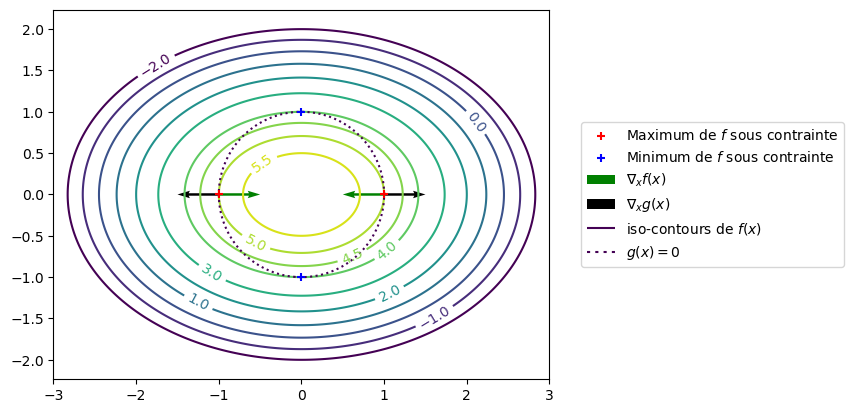
\includegraphics[width=0.95\linewidth]{Images/multiplicateurs_lagrange}
		\label{fig:multiplicateurs_lagrange}
	\end{figure}
\end{frame}